\section{Conclusion}



\begin{frame}<handout:0>[noframenumbering]
  \begin{overlay}
    \sectionCircle
  \end{overlay}
\end{frame}



\subsection{Conclusion}

\begin{frame}{\insertsubsection}
  \begin{overlay}
    \node[anchor=center] at (80,42.912) {%
      \includegraphics[height=50mm]{glasses}};
  \end{overlay}
\end{frame}

{
  \setbeamertemplate{footline}{}
  \begin{frame}[noframenumbering]
    \begin{overlay}
      \node[anchor=center] at (80,45) {%
        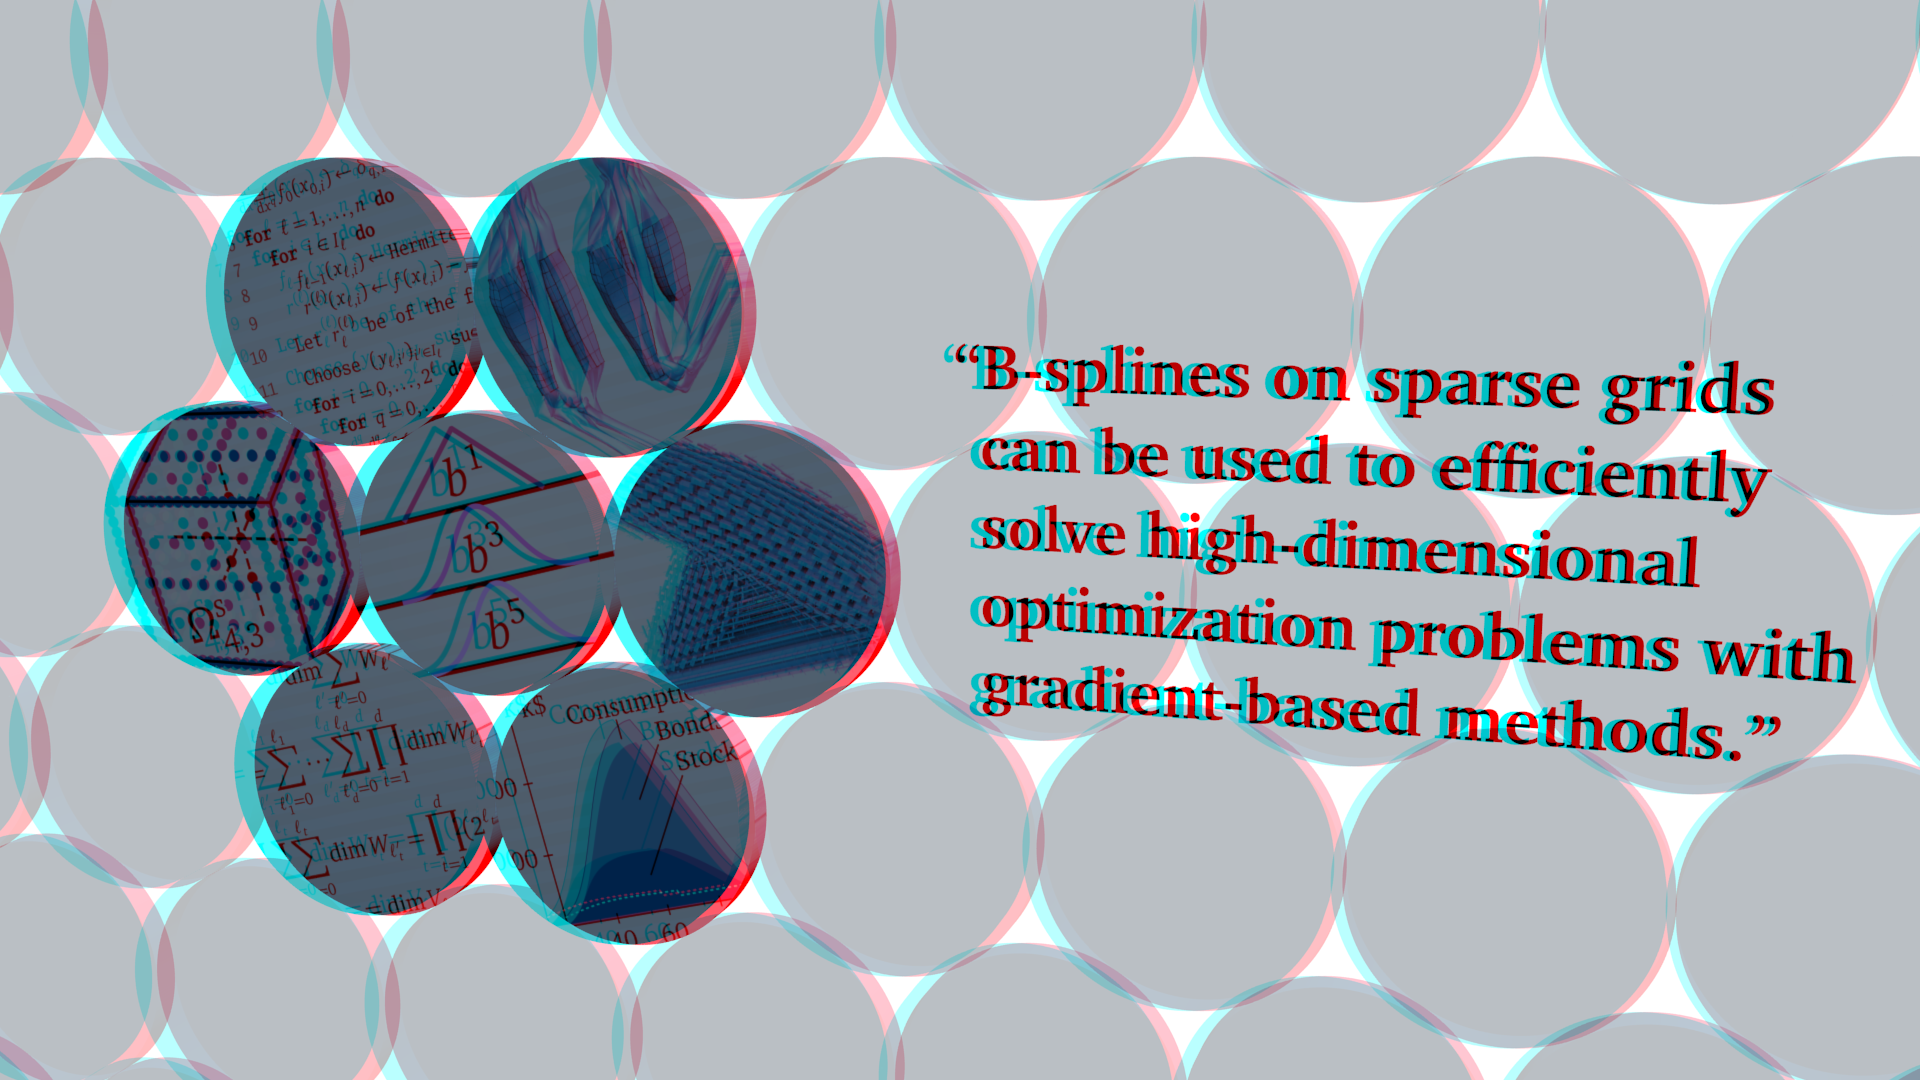
\includegraphics[scale=\pngscale]{message}%
      };
    \end{overlay}
  \end{frame}
}



\subsection{Literature (Published)}

\begin{frame}{\insertsubsection}
  \begin{itemize}
    \item
    \fullcite{Pflueger16Scalability}
    
    \item
    \fullcite{Valentin16Hierarchical}
    
    \item
    \fullcite{Valentin18Fundamental}
    
    \item
    \fullcite{Valentin18Gradient}
  \end{itemize}
\end{frame}



\subsection{Literature (In Preparation)}

\begin{frame}{\insertsubsection}
  \begin{itemize}
    \item
    \fullcite{Pflueger19Solving}
    
    \item
    \fullcite{Valentin19Gradient}
    
    \item
    \fullcite{Valentin19Boundary}
  \end{itemize}
\end{frame}



\subsection{Literature (Supplemental)}

\begin{frame}{\insertsubsection}
  \begin{itemize}
    \item
    \fullcite{Feynman11Mainly}
    
    \item
    \fullcite{Valentin12Spline}
    
    \item
    \fullcite{Valentin14Hierarchische}
  \end{itemize}
\end{frame}
